\csname documentclass\endcsname[../main.tex]{subfiles}
\graphicspath{{\subfix{../images/}}}
\begin{document}

This section provides an overview of ITSs with an emphasis on congestion management, reviews techniques for traffic forecasting (from classical time-series models to modern machine learning approaches), discusses congestion management strategies (distinguishing reactive and proactive methods such as adaptive signalling, dynamic rerouting, and speed control), outlines the role of traffic simulation tools (e.g. SUMO and TraCi) in evaluating traffic control strategies, and finally identifies research gaps that motivate the development of a proactive, data-driven congestion management system.

\subsection{Intelligent Transportation Systems}

ITSs are typical in today’s smart infrastructure. These refer to the use of advanced information and communication technologies in transport infrastructures to reduce traffic congestion, improve road safety, and increase the overall efficiency of traffic networks. ITSs have quickly evolved over the past few decades from isolated, low-capability systems to integrated networks of adaptive systems with much more significant impact. These use a variety of sensors, communication forms, and efficient computing capabilities for traffic management.

\paragraph{Deployment.} These modern ITSs are typically deployed with an array of road sensors (such as inductive loops, cameras, and radar) and communication mechanisms. Centralised traffic management centres then enable the continuous monitoring and control of the networks \cite{office_intelligent_nodate}. For instance, an example of an ITS is detectors on roads that feed real-time traffic data to the control centre, where operators can check conditions (often using CCTV feeds) and then respond accordingly by adjusting control devices such as traffic light timing \cite{a_kurdi_review_2014}. A diagram of a typical ITS is shown in \fig{ITS}.

\begin{figure}[!ht]
  \centering
  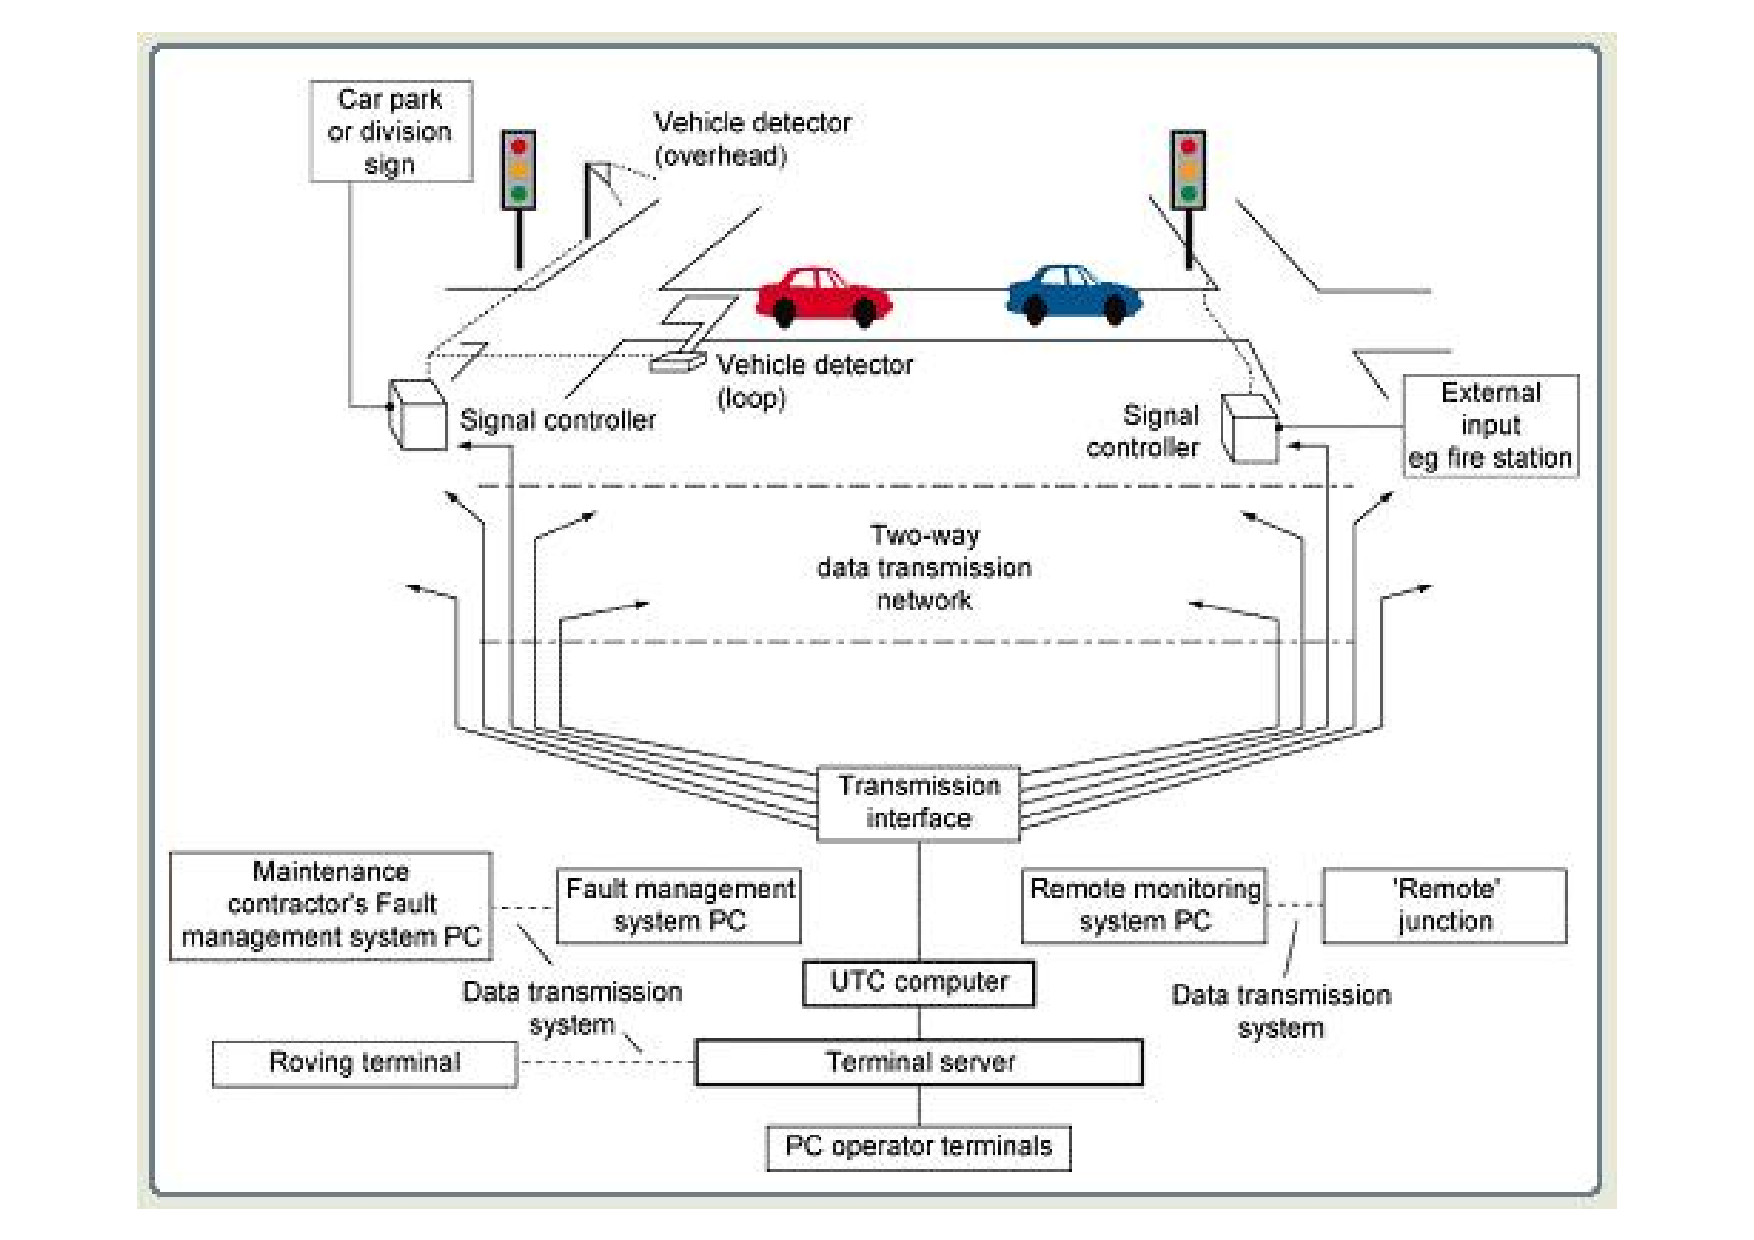
\includegraphics[width=0.7\textwidth]{images/background/ITS.pdf}
  \caption[The flow of information in SCOOT based UTC system - an example of an ITS]{The flow of information in SCOOT based UTC system - an example of an ITS from~\cite{noauthor_urban_nodate}}
  \label{fig:ITS}
\end{figure} 

Modern ITS systems can automatically implement congestion management strategies. These include adaptive signal control systems that adjust traffic light timing in response to traffic conditions, ramp metering systems that regulate the entry of vehicles to highways, or traveller information systems that inform drivers about road conditions and alternative routes \cite{noauthor_what_nodate}.

\paragraph{Performance.} These technologies have been shown to reduce delays and improve network performance; for example, adaptive signal control has been documented to smooth traffic flow, reducing delay by optimising signal timing in real-time \cite{zhao_overview_2012}. In many congested metropolitan areas, multiple ITS technologies are deployed in conjunction – a traffic management centre may simultaneously utilise detection systems, coordinated signals, dynamic speed limit signs, and route guidance, each addressing different aspects of congestion. The overall trend in ITSs is toward increasingly integrated and intelligent systems, allowing a focus on more proactive traffic management approaches.

Despite these advancements, most current ITS implementations still function reactively, responding to congestion or incidents as they occur. These typically detect congestion (via connected sensors) and then trigger control measures to mitigate it. While these approaches are efficient, reacting after queues have formed may not always be fast or compelling enough to prevent traffic buildup and congestion. This limitation in the most used current ITSs motivates the incorporation of predictive analytics and proactive control, as discussed later in this section.


\subsection{Traffic Forecasting}
Accurate traffic forecasting is an essential mechanism to allow for advanced traffic management. While not a standalone solution, traffic forecasting enables proactive traffic control by informing decisions. Many real-world applications currently use predictions in some form. For example, navigation services (Google Maps, Waze) use traffic forecasting to predict travel times on routes to inform drivers of route choices \cite{noauthor_google_2020}, and traffic authorities use predicted traffic volumes to reactively enable measures such as ramp metering or variable message signs. However, fully taking advantage of the power of traffic forecasting within ITS is still a work in progress. 

\subsubsection{Time-Series Forecasting (ARIMA)}
Traditional approaches to traffic prediction rely on time-series modelling techniques. Among these, the \abbrev{Auto-Regressive Integrated Moving Average}{ARIMA} model and its variants have been widely adopted for traffic flow and travel time prediction, albeit only for short-term predictions. These older models are based on more traditional statistical methods and have proven to capture recurring patterns in historical traffic data and are often used as a baseline for traffic forecasting \cite{katambire_forecasting_2023}.

In practice, however, these types of models (purely statistical) have severe limitations: they are essentially only useful for short-term forecasts; they assume linear relationships in the time series and, therefore, struggle to model the complex, nonlinear structure of trends inherent in the transport networks.

\subsubsection{Machine Learning and Neural Network Techniques}
In recent years, as with most domains, machine learning approaches have gained dominance in traffic forecasting due to their ability to model much deeper trends and accept many data sources. The feed-forwards \abbrev{Multi-Layer Perceptron}{MLP} is a common approach that learns direct mappings from past data. A simplified architecture diagram of the MLP is shown in \fig{MLP}.

\begin{figure}[!ht]
  \centering
  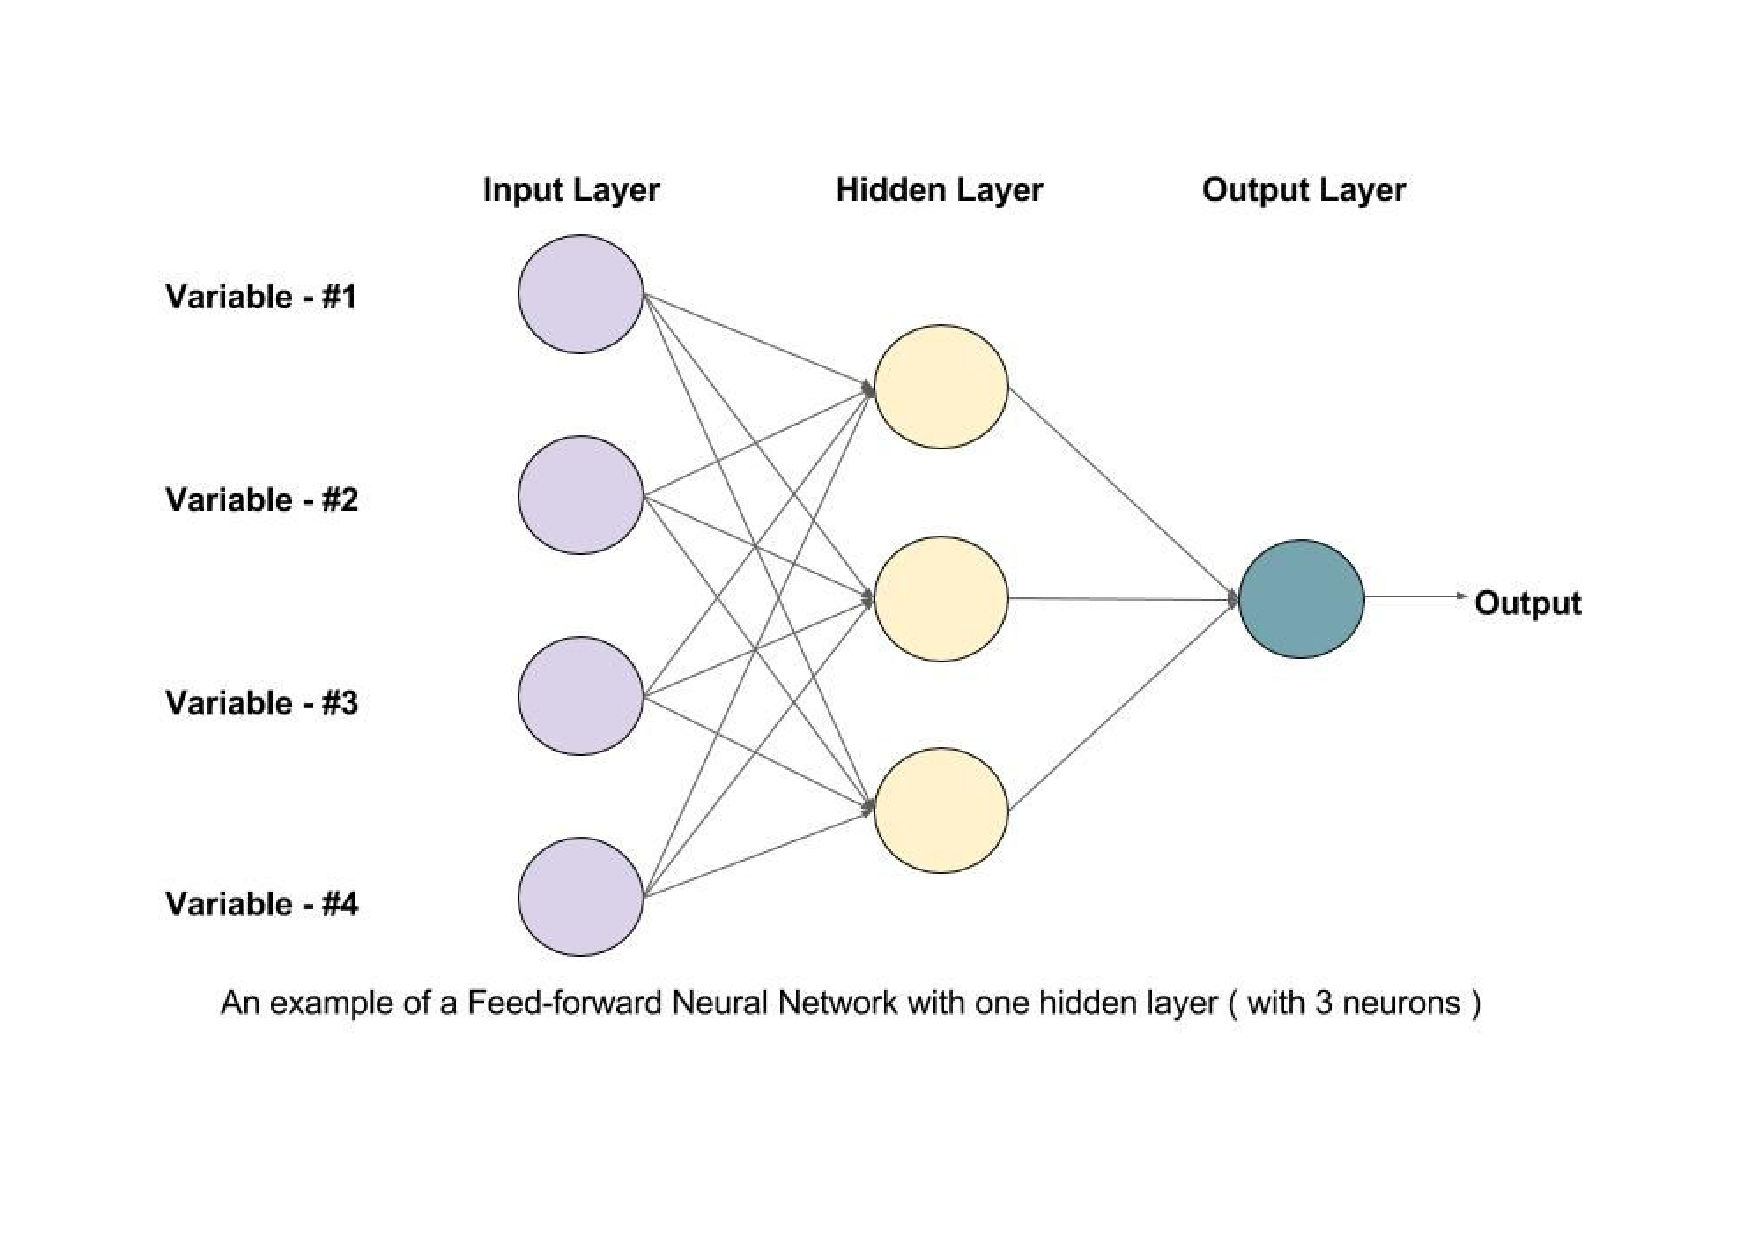
\includegraphics[width=0.7\textwidth]{images/background/mlp.pdf}
  \caption[A simplified MLP architecture diagram]{A simplified MLP architecture diagram from~\cite{gupta_understanding_2017}}
  \label{fig:MLP}
\end{figure} 

\paragraph{Multi-Layer Perceptron (MLP).} MLPs and other artificial neural networks have been successfully applied to predict traffic conditions, showing improved accuracy over the traditional models. For example, a team of researchers compared several predictive models (including linear and polynomial regression, radial-basis function network, and a feed-forward neural network) for congestion prediction based on several inputs such as traffic waiting times, time-of-week indicators and holidays \cite{noauthor_traffic_nodate}. They achieved the highest accuracy with the neural network at about 97.6\%, outperforming all the other techniques. Their research demonstrates the effectiveness of even simpler neural networks (such as MLPs) when used with rich input features.

\paragraph{Recurrent Neural Networks (RNNs).} More sophisticated machine learning models may improve predictive performance for specific applications. In particular, \abbrev{Recurrent Neural Network}{RNN}s and their variants, like \abbrev{Long Short-Term Memory}{LSTM} networks, have shown great performance in traffic forecasting. A simplified architecture diagram of a LSTM network is shown in \fig{LSTM}. LSTMs are designed to retain long-term dependencies and handle time-varying patterns such as seasonally well. However, these networks suffer from vanishing gradients and difficulties retaining distant dependencies, making them inefficient for long-term forecasting, just like the ARIMA models. Numerous studies have found LSTM-based predictors to outperform traditional models such as ARIMA on various traffic metrics. For instance, Katambire \textit{et al.} (2023) deployed an LSTM and an ARIMA model to forecast traffic volumes at a busy urban junction. The results indicated that the LSTM was the best-fitting model for predicting monthly traffic flow, exceeding the accuracy of the ARIMA approach \cite{katambire_forecasting_2023}.

\begin{figure}[!ht]
  \centering
  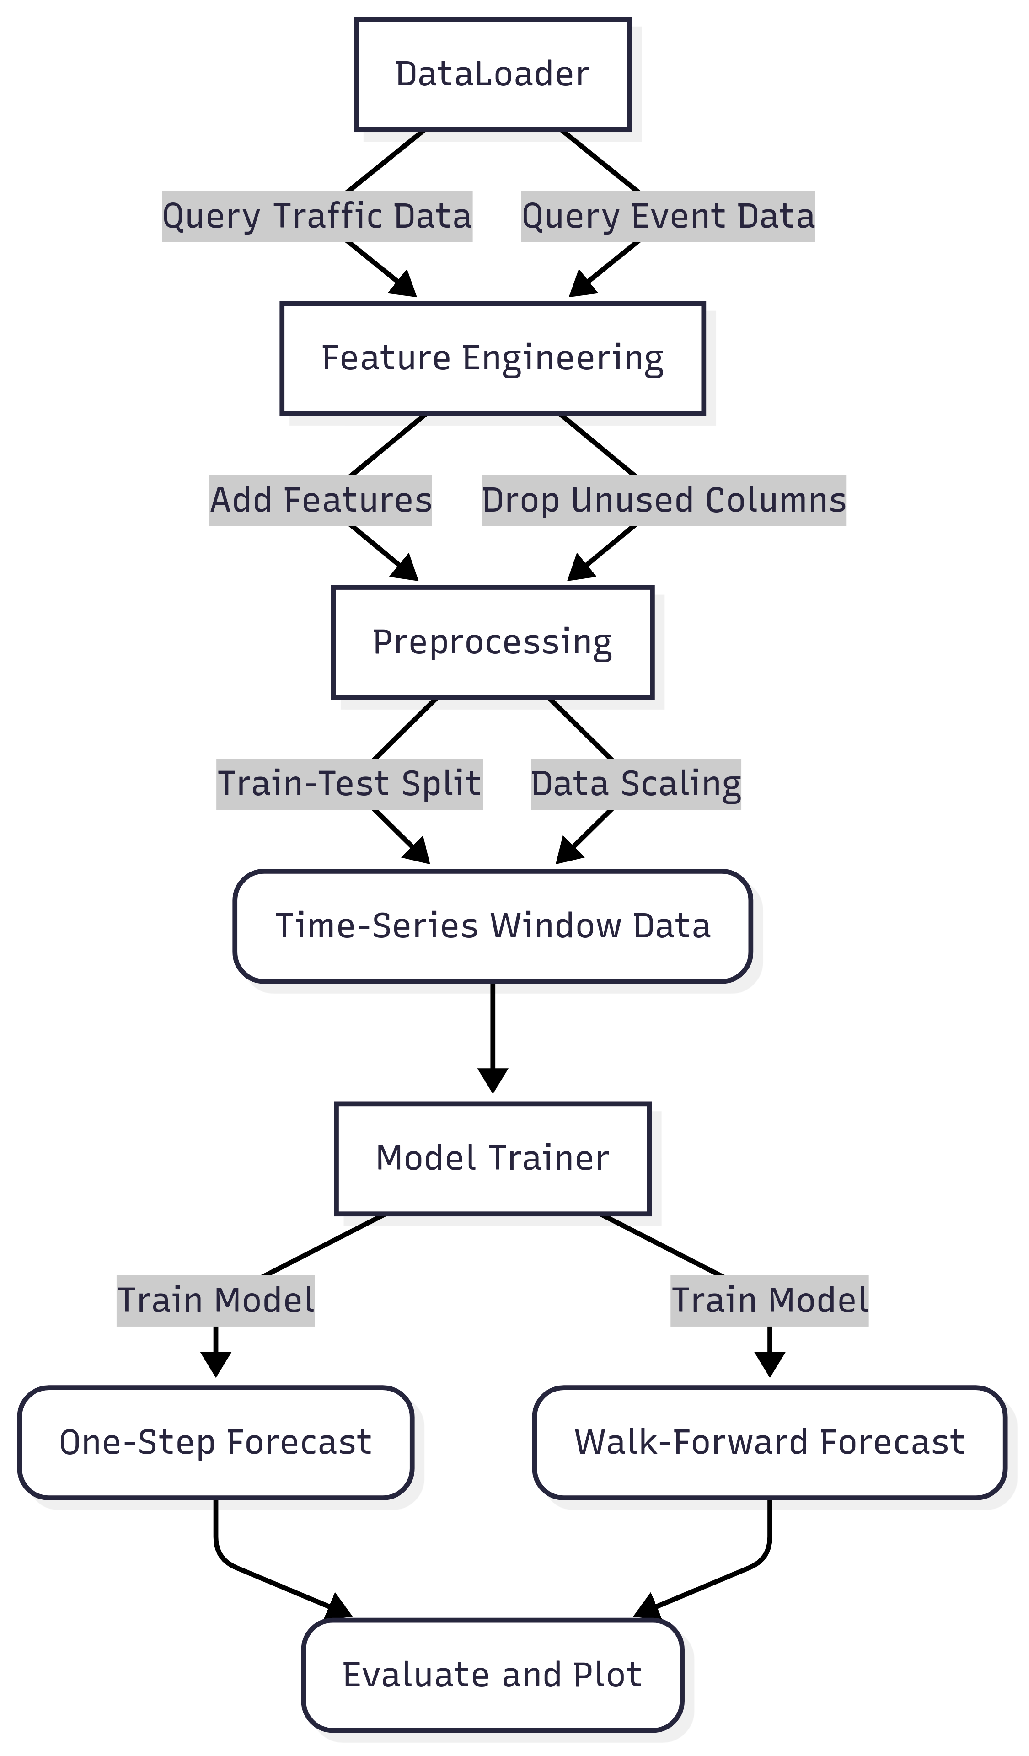
\includegraphics[width=0.7\textwidth]{images/background/lstm.pdf}
  \caption[A simplified LSTM architecture diagram]{A simplified LSTM architecture diagram from~\cite{yan_understanding_2017}}
  \label{fig:LSTM}
\end{figure} 

\subsubsection{Recent Advancements}
\paragraph{Hybrid Aproaches.} Beyond individual models, researchers have recently explored hybrid and deep learning architectures to push predictive accuracy. One strategy is combining two models to their strengths, such as coupling an ARIMA model (that excels at capturing linear trends) with an MLP (great at nonlinear patterns). This type of combination can improve prediction accuracy compared to the standalone models \cite{v_hybrid_2022}.

\paragraph{Deep Learning Approaches.} For long-term forecasting, recent advanced approaches incorporate spatial information, treating the traffic network as a graph of sensors and road segments. When doing so with \abbrev{Graph Neural Network}{GNN}s or \abbrev{Convolutional Neural Network}{CNN}s on spatio-temporal data, they show excellent adaptive performance to model interconnected congestion patterns by learning how congestion at one location influences another \cite{jiang_graph_2022, ma_learning_2017}. Broadly, machine learning techniques (from basic MLPs to complex LSTM and graph networks) have significantly improved predictive accuracy and are increasingly being integrated into traffic management systems \cite{kumar_applications_2021}.

\subsection{Congestion Management Approaches}
\label{link:cmt}
Traffic congestion management strategies can typically be classified into two categories: reactive and proactive approaches. In the next subsections, we will review examples of each, highlight the traditional ITS approach of reacting to congestion, and discuss how emerging methods aim to predict and avert congestion before it occurs.

\subsubsection{Reactive Methods}
Reactive congestion management is the most traditional strategy, responding to traffic conditions or incidents as they occur to reduce congestion or contain it after it has already developed. Most conventional ITS implementations fall into this category. These systems continuously monitor traffic (for example, through loop detectors and cameras) and trigger control actions when congestion is detected, or traffic density thresholds are exceeded. A typical example is adaptive signal control, where traffic signal timings (green/red phases) are adjusted based on volumes at intersections. If an intersection becomes congested, the controller can extend the green time on the most congested approach to clear it. This type of system has been consistently deployed worldwide and has been shown to reduce delays by smoothing the flow through intersections \cite{office_intelligent_nodate}. 
Other examples of these methods include \cite{office_intelligent_nodate}:
\begin{itemize}
    \item \textbf{\abbrev{Variable Speed Limit}{VSL}:} Reduced speed limits prevent shockwave formation when congestion occurs.
    \item \textbf{Dynamic Rereouting:} Drivers are alerted to congestion through dynamic signs or GPS systems and rerouted to avoid the congestion.
    \item \textbf{Ramp Metering:} Controls the flow of vehicles entering a motorway to improve traffic flow.
\end{itemize}

These reactive methods are significant components in current ITSs and have proven effective to an extent: by responding in real-time, they can reduce the duration and severity of congestion. However, the major limitation of these approaches is that they wait for congestion to occur before taking action. In scenarios of fast-rising demand (for example, the sudden influx of cars after a stadium event ends), purely reactive control might not be sufficient or act too late, as the congestion would have already built up by the time the system intervenes.

\subsubsection{Proactive Methods}
Proactive congestion management aids in covering the inefficiencies of reactive methods by predicting or anticipating traffic conditions and taking control actions in advance. This approach uses predictive analytics (like the earlier forecasting models) that are tightly integrated with traffic control algorithms. The systems continuously generate forecasts of traffic state for various, often critical, intersections and roads, looking slightly ahead. If congestion is predicted to build up soon, the system proactively implements control measures before the congestion fully occurs. These usually include the same strategies as in reactive control (signals, routing, adaptive speed limits), but the timing is guided by predictions rather than current measurements.

Using the same example of predictive signal control, the system would preemptively adjust green phases to accommodate surges just before they occur, reroute drivers in advance of a stadium match ending, or reducing speed limits just before a high influx of traffic.

\paragraph{Feasibility.} The feasibility of proactive traffic management has recently greatly improved due to advances in both computing power and predictive models. Some research prototypes have successfully demonstrated that integrating traffic prediction control is possible and beneficial. For example, a recent study funded by the U.S. Federal Highway Administration developed a prototype system with traffic prediction and a reinforcement learning engine to recommend traffic control interventions \cite{us_department_of_transportation_federal_highway_administration_predictive_nodate}. This system could analyse real-time data and learn optimal interventions. At a city scale, the city of Groningen in the Netherlands piloted a similar system that combined traffic prediction with an adaptive control platform \cite{noauthor_predictive_nodate}. These examples demonstrate the potential of proactive methods to improve congestion management in continuously denser urban environments.

\paragraph{Reactive \& Proactive Interplay.} We note, however, that proactive strategies do not replace reactive ones but should enhance them. Even in proactive systems, reactive adjustments will still be needed for unforeseen traffic events (such as crashes). The proactive congestion management area is still emerging, and deployments are not yet typical, mainly due to the challenges in obtaining reliable predictions and the complexity of the decision-making algorithms required. Nonetheless, as we will discuss later, the growing computing capabilities, abundant available data, and modern machine learning algorithms provide a strong direction to enable proactive congestion management algorithms.

\subsection{Traffic Simulation}
Before new traffic control strategies can be implemented on real roads, they must be thoroughly tested. Traffic simulation tools play a crucial role in this process, allowing researchers and traffic engineers to model real-world traffic dynamics in a virtual environment. This allows new approaches to be tested without risk or costly field experiments. These tools replicate the behaviour of individual vehicles and their interactions on road networks, providing detailed insights into how congestion develops and to what extent control measures are effective.

A variety of traffic simulation software packages have been developed, ranging from commercial products like VISSIM and Aimsun to open-source platforms like SUMO and VEINS (which couples SUMO with a communication network simulator OMNeT++).

\subsubsection{Simulation of Urban MObility (SUMO)}
\abbrev{Simulation of Urban MObility}{SUMO}, in particular, has become popular in academic and research settings as a flexible, microscopic traffic simulator capable of handling large networks \cite{krajzewicz_traffic_2010}. It allows the modelling of each vehicle’s movement through road networks with user-defined routes and supports the simulation of various transportation modes (such as cars, buses, and pedestrians). An example SUMO simulation is shown in \fig{SUMO_example}.

\begin{figure}[!ht]
  \centering
  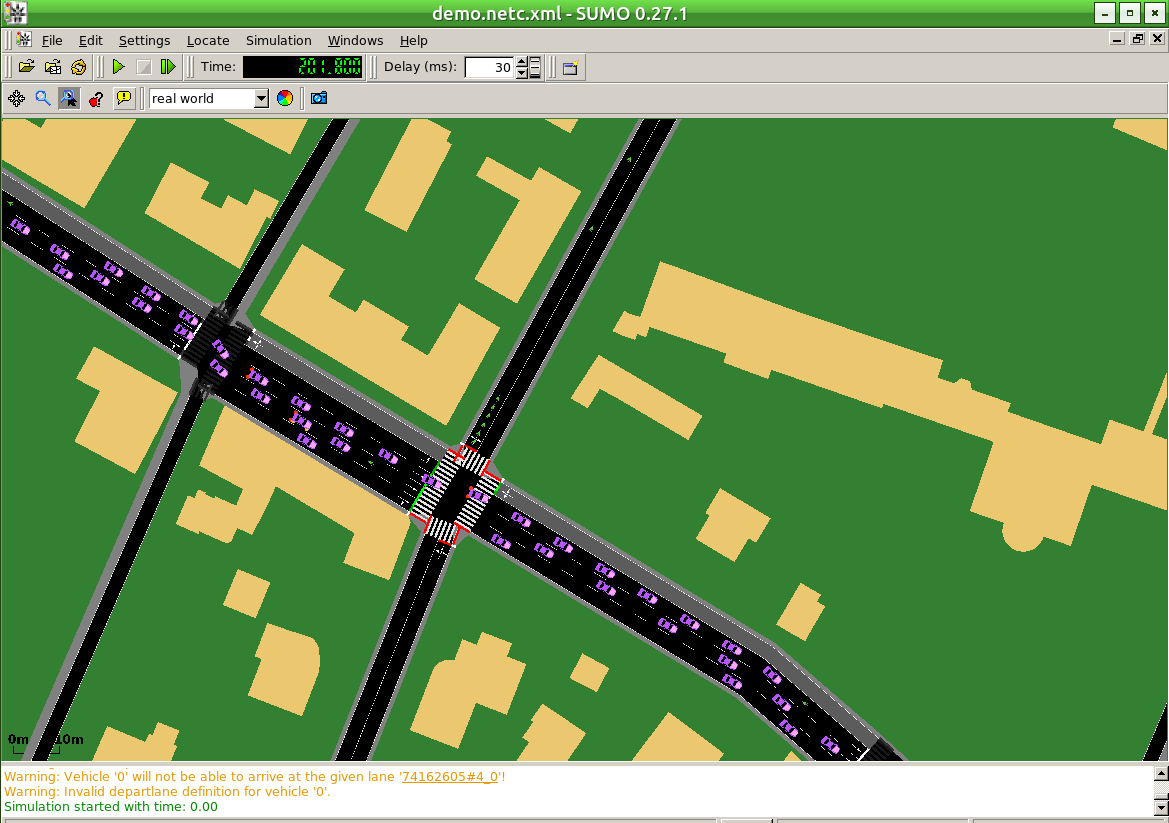
\includegraphics[width=0.7\textwidth]{images/background/sumo_example.png}
  \caption[An example SUMO simulation]{An example SUMO simulation from~\cite{noauthor_getting_nodate}}
  \label{fig:SUMO_example}
\end{figure} 

One of the key advantages of SUMO is that it is open-source and highly customisable. It is, for example, frequently used to evaluate adaptive signal control algorithms by simulating a city’s intersection and testing how the control algorithms impact queues and travel times \cite{krajzewicz_traffic_2010}. Crucially, SUMO provides not just average performance metrics (such as total network delay) but also fine-grained metrics of traffic, which help tune parameters and investigate issues.

\subsubsection{Traffic Control Interface (TraCi)}
An important feature of SUMO (and several other modern simulators) is the ability to interact with the simulation in real time through an API. In SUMO’s case, this is facilitated by \abbrev{Traffic Control Interface}{TRaCi}, which is a network-based interface that allows an external program (such as using Python) to query and control the state of the simulation at each time step \cite{krajzewicz_traffic_2010}. Using this API, we can retrieve fine-grained information from the simulation and send actions back in response as the simulation runs.

This capability makes SUMO powerful for testing closed-loop traffic management algorithms like the ones in this project’s scope. As a concrete example, the proactive traffic management prototype mentioned earlier (by the U.S. Federal Highway Administration) was evaluated using a similar setup of emulated real traffic scenarios, allowing researchers to verify that their algorithms led to improvements compared to a baseline \cite{us_department_of_transportation_federal_highway_administration_predictive_nodate}.

\subsection{Research Gaps}

The literature reviewed above shows strong progress in traffic sensing, modelling, and control, but there remain key gaps, particularly in how these domains are combined in real-world systems.

\subsubsection{Predictive Model Integration}

ITS deployments increasingly include complex monitoring and reactive control. However, most systems still rely only on real-time data, with limited use of predictive models for proactive congestion management. For instance, motorway ramp meters typically respond to current occupancy, and adaptive signal systems like SCOOT or SCATS adjust to measured queues but do not forecast future congestion \cite{stevanovic_scoot_2009}. Despite research showing the benefits of predictive control, deployments are rare due to integration challenges and a reluctance to act on uncertain forecasts. Closing this gap requires not just accurate prediction but also practical evidence that such predictions can be trusted in live environments.

\subsubsection{Importance of External Contextual Data}

A second gap lies in incorporating external contextual data, particularly large-scale event information, into traffic prediction and control. Congestion is not driven by traffic dynamics alone. Events such as football matches and concerts can cause significant, location-specific spikes in demand. While some research has explored this, such as Kwoczek \textit{et al.} (2014) who showed a 35\% improvement when incorporating event data in Cologne \cite{kwoczek_predicting_2014}, these efforts often rely on ad hoc data collection and are rarely operationalised in ITS. Most real-world systems still handle such scenarios manually, if at all.

\subsubsection{Project Positioning and Justification}
This project directly addresses both gaps. We develop a predictive model that integrates traffic sensor data, temporal features, and large-scale event information to forecast congestion ahead of time. This is combined with a proactive control method, specifically, a VSL-based congestion management strategy—that uses these predictions to intervene before congestion forms. This pairing is motivated by prior work showing the benefits of contextual data, and by our evaluation, which demonstrates that integrating prediction and control produces measurable improvements, confirmed by simulation. Further design decisions, including model structure and control logic, are detailed in \textbf{\hyperref[sec:design-implementation]{Section 3}}.

\end{document}
